\setcounter{section}{2}
\section{Normen und Skalarprodukte}

\subsection{Normen}

Bisher haben wir mit den Vektorräumen die Vektoroperationen verallgemeinert. Wir wissen also wie wir, unabhängig von den Objekten in einem Vektorraum rechnen können. Nun wollen wir einen weiteren Schritt machen und die Grösse von Vektoren aus einem Vektorraum vergleichen. Dafür ordnen wir jedem Vektor \( v \), in einem Vektorraum, eine reelle positive Zahl zu, da wir deren Grösse gut vergleichen können, z.B. können wir ganz klar sagen, dass die Zahl 6 grösser als die Zahl 3 ist. 

\vspace{1\baselineskip}

\begin{figure}[h!]
    \centering
    \tikzset{every picture/.style={line width=0.75pt}} %set default line width to 0.75pt  
    \tikzsetnextfilename{norm_zahl_strahl}       
    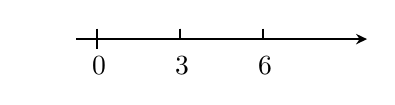
\begin{tikzpicture}[x=0.75pt,y=0.75pt,yscale=-1,xscale=1]
        %uncomment if require: \path (0,300); %set diagram left start at 0, and has height of 300
        %Straight Lines [id:da9386888791038366] 
        \draw    (260,70) -- (397,70) ;
        \draw [shift={(400,70)}, rotate = 180] [fill={rgb, 255:red, 0; green, 0; blue, 0 }  ][line width=0.08]  [draw opacity=0] (5.36,-2.57) -- (0,0) -- (5.36,2.57) -- (3.56,0) -- cycle    ;
        %Straight Lines [id:da23632381199419694] 
        \draw    (310,65) -- (310,70) ;
        %Straight Lines [id:da47899723805415684] 
        \draw    (350,65) -- (350,70) ;
        %Straight Lines [id:da21722339296341664] 
        \draw    (270,65) -- (270,70) ;
        %Straight Lines [id:da2629189072272182] 
        \draw    (310,65) -- (310,70) ;
        %Straight Lines [id:da7141794096730381] 
        \draw    (270,70) -- (270,75) ;
        % Text Node
        \draw (306,77) node [anchor=north west][inner sep=0.75pt]   [align=left] {$\displaystyle 3$};
        % Text Node
        \draw (346,77) node [anchor=north west][inner sep=0.75pt]   [align=left] {$\displaystyle 6$};
        % Text Node
        \draw (266,77) node [anchor=north west][inner sep=0.75pt]   [align=left] {$\displaystyle 0$};
        % Text Node
        \draw (237,68) node [anchor=north west][inner sep=0.75pt]  [font=\small] [align=left] {$\displaystyle \dotsc $};
    \end{tikzpicture}
\end{figure}

\vspace{0.5\baselineskip}

Wie sieht es jedoch mit Vektoren aus? Hier ist die Antwort nicht so offensichtlich. Welcher dieser Vektoren ist grösser?

\begin{figure}[h!]
    \centering
    \tikzset{every picture/.style={line width=0.75pt}} %set default line width to 0.75pt  
    \tikzsetnextfilename{norm_zwei_vektoren}       
    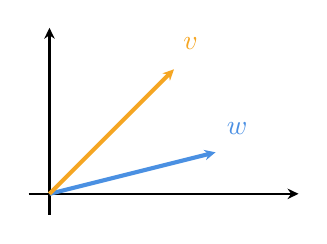
\begin{tikzpicture}[x=0.75pt,y=0.75pt,yscale=-1,xscale=1]
        %uncomment if require: \path (0,300); %set diagram left start at 0, and has height of 300
        %Straight Lines [id:da728200412340026] 
        \draw    (260,120) -- (387,120) ;
        \draw [shift={(390,120)}, rotate = 180] [fill={rgb, 255:red, 0; green, 0; blue, 0 }  ][line width=0.08]  [draw opacity=0] (5.36,-2.57) -- (0,0) -- (5.36,2.57) -- (3.56,0) -- cycle    ;
        %Straight Lines [id:da4702091733424284] 
        \draw    (270,130) -- (270,43) ;
        \draw [shift={(270,40)}, rotate = 90] [fill={rgb, 255:red, 0; green, 0; blue, 0 }  ][line width=0.08]  [draw opacity=0] (5.36,-2.57) -- (0,0) -- (5.36,2.57) -- (3.56,0) -- cycle    ;
        %Straight Lines [id:da9389986271719671] 
        \draw [color={rgb, 255:red, 74; green, 144; blue, 226 }  ,draw opacity=1 ] [line width=1.5]  (270,120) -- (347.09,100.73) ;
        \draw [shift={(350,100)}, rotate = 165.96] [fill={rgb, 255:red, 74; green, 144; blue, 226 }  ,fill opacity=1 ][line width=0.08]  [draw opacity=0] (5.36,-2.57) -- (0,0) -- (5.36,2.57) -- (3.56,0) -- cycle    ;
        %Straight Lines [id:da4329019838984933] 
        \draw [color={rgb, 255:red, 245; green, 166; blue, 35 }  ,draw opacity=1 ] [line width=1.5]  (270,120) -- (327.88,62.12) ;
        \draw [shift={(330,60)}, rotate = 135] [fill={rgb, 255:red, 245; green, 166; blue, 35 }  ,fill opacity=1 ][line width=0.08]  [draw opacity=0] (5.36,-2.57) -- (0,0) -- (5.36,2.57) -- (3.56,0) -- cycle    ;
        % Text Node
        \draw (333,43) node [anchor=north west][inner sep=0.75pt]  [color={rgb, 255:red, 245; green, 166; blue, 35 }  ,opacity=1 ] [align=left] {$\displaystyle v$};
        % Text Node
        \draw (354,84) node [anchor=north west][inner sep=0.75pt]  [color={rgb, 255:red, 245; green, 166; blue, 35 }  ,opacity=1 ] [align=left] {$\displaystyle \textcolor[rgb]{0.29,0.56,0.89}{w}$};
    \end{tikzpicture}
\end{figure}

\begin{equation*}
    v = \begin{pmatrix} 3 \\ 3 \end{pmatrix} \ \text{oder} \ w = \begin{pmatrix} 4 \\ 1 \end{pmatrix}.
\end{equation*}

\vspace{0.25\baselineskip}

Nun kommt es darauf an was grösser in diesem Kontext bedeutet z.B.\ könnte man argumentieren, dass:

\begin{itemize}
    \item \( v \) ist grösser, da die geometrische Länge grösser ist.
    \item \( w \) ist grösser, da der Vektor eine grössere Zahl enthält.
\end{itemize}

Normen werden uns nun helfen diese Frage eindeutig zu beantworten. Denn eine Norm ist eine fixe Regel, mit welcher man jedem Vektor eine reelle positive Zahl zuordnen kann. Dadurch kann man Sie dann vergleichen. Mathematisch lässt sich das durch eine Abbildung ausdrücken:

\begin{equation*}
    \| {\cdot} \| : V \rightarrow \mathbb{R}, \quad v \mapsto \| v \|.
\end{equation*}

\vspace{0.25\baselineskip}

Wie im Beispiel von oben, gibt es viele Möglichkeiten diese Zuordnung zu machen. 

\begin{itemize}
    \item Geometrische Länge (Euklidische Norm)
        \begin{equation*}
            \begin{aligned}
                \| x \|_2 = \sqrt{x_1^2 + x_2^2} \quad \to \quad \| v \|_2 &= \sqrt{18} \\
                \| w \|_2 &= \sqrt{17}
            \end{aligned}        
        \end{equation*}
    \item grösster Eintrag (Maximumsnorm)
        \begin{equation*}
            \begin{aligned}
                \| x \|_\infty = \max \{ |x_1|, |x_2| \} \quad \to \quad \| v \|_\infty &= 3 \\
                \| w \|_\infty &= 4
            \end{aligned}        
        \end{equation*}
\end{itemize}

Achtung! Nicht alles ist eine Norm, es müssen bestimmte Bedingungen erfüllt sein damit eine Norm vorhanden ist.

\begin{tcolorbox}[colback=gray!30, colframe=gray!80, title=Vektornormen]
    Eine Norm ordnet jedem Vektor eine reelle Zahl zu und kann so als eine Art Mass verstanden werden.\ \( \forall v, w \in V, \alpha \in \mathbb{R} \) muss gelten:
    \begin{equation*}
        \begin{aligned}
            & \| v \| \geq 0 \ \text{und} \ \| v \| = 0 \Leftrightarrow v = 0 \\[0.5em]
            & \| \alpha \cdot v \| = |\alpha| \cdot \| v \| \\[0.5em]
            & \| v + w \| \leq \| v \| + \| w \|
        \end{aligned}
    \end{equation*}
\end{tcolorbox}

\vspace{0.5\baselineskip}

Beispiele solcher Normen sind:

\begin{equation*}
    \text{Auf} \ \mathbb{R}^n \left\{ 
    \begin{array}{ll}  
        \| v \|_2 := \sqrt{v_1^2 + \cdots + v_n^2} \quad &\text{(Euklidische Norm)}\\[0.75em]
        \| v \|_\infty := \max \{ |v_1|, \ldots, |v_n| \} \quad &\text{(Maximumsnorm)}\\[0.75em]
        \| v \|_p := \left( |v_1|^p + \cdots + |v_n|^p \right)^{\frac{1}{p}} \quad &(p\text{-Norm}, 1\leq p < \infty)
    \end{array}
\right. 
\end{equation*}

\vspace{0.5\baselineskip}

\begin{equation*}
    \text{Auf} \ \mathbb{R}^{n \times m} \left\{ 
    \begin{array}{ll}  
        \| A \|_2 := \sqrt{\sum_{i,j}|a_{ij}|^2} \quad &\text{(Hilbert-Schmidt-Norm)}\\[0.75em]
        \| A \|_{\text{SM}} := \underset{1 \leq j \leq n}{\max} \sum_{i=1}^{m} | a_{ij} | \quad &\text{(Spaltenmaximumsnorm)}\\[0.75em]
        \| A \|_{\text{ZM}} := \underset{1 \leq i \leq m}{\max} \sum_{j=1}^{n} | a_{ij} | \quad &\text{(Zeilenmaximumsnorm)}
    \end{array}
\right. 
\end{equation*}

\subsection{Skalarprodukte}

Wir haben nun einen Weg um die Grösse von Vektoren in einem Vektorraum zu vergleichen. Im nächsten Schritt wollen wir die Beziehung zwischen zwei Vektoren mit einer reellen Zahl beschrieben. Wieder lässt sich dies durch eine Abbildung beschreiben. 

\begin{equation*}
    \langle \cdot, \cdot \rangle : V \times V \rightarrow \mathbb{R}, \quad (x, y) \mapsto \langle x, y \rangle.
\end{equation*}

\vspace{0.5\baselineskip}

Auch hier müssen bestimmte Bedingungen erfüllt sein.

\begin{tcolorbox}[colback=gray!30, colframe=gray!80, title=Skalarprodukte]
    Ein Skalarprodukt ordnet jedem Vektorpaar eine reelle Zahl zu, diese beschreibt die Beziehung der beiden Vektoren zueinander.\ \( \forall x, y, z \in V, \alpha \in \mathbb{R} \) muss gelten:
    \begin{equation*}
        \begin{aligned}
            & \langle x, y + z \rangle = \langle x, y \rangle + \langle x, z \rangle \\[0.5em]
            & \langle x, \alpha \cdot y \rangle = \alpha \cdot \langle x, y \rangle \\[0.5em]
            & \langle x, y \rangle = \langle y, x \rangle \\[0.5em]
            & \langle x, x \rangle \geq 0 \ \text{und} \ \langle x, x \rangle = 0 \Leftrightarrow x = 0
        \end{aligned}
    \end{equation*}
\end{tcolorbox}

\vspace{0.5\baselineskip}

Wenn \( \langle x, y \rangle = 0 \), dann sind \( x, y \) orthogonal zueinander \( (x \perp y) \). 

\subsection{Vom Skalarprodukt induzierte Norm}

Das Skalarprodukt kann auch benutzt werden, um eine Norm zu induzieren. Wenn auf einem Vektorraum ein Skalarprodukt gegeben ist, kann daraus direkt eine Norm der Form

\begin{equation*}
    \| x \| := \sqrt{\langle x, x \rangle}
\end{equation*}

abgeleitet werden. Diese Norm erfüllt automatisch alle Bedingungen einer Norm, egal welches Skalarprodukt benutzt wird. 